\chapter{Effect of regional-scale forest species conversion on the atmospheric boundary layer in the Northern California Coast Range}
\label{c.BL}

\textbf{Abstract:}  Common evergreen tree species in Northern California respond to summer drought with different water use strategies.  In this study, the effect of these different water use patterns on the atmospheric boundary layer is estimated, using two atmospheric models, one simple and one comprehensive.  Two tree species with very different water use strategies are tested, in order to quantify the maximum impact of species distribution on the dry season atmosphere, using extreme regional-scale scenarios of complete forest species conversion from 100\% Douglas fir (\textit{Pseudotsuga menziesii}) to 100\% Pacific madrone (\textit{Arbutus menziesii}).  For representative mid-summer periods, atmospheric boundary layer conditions (temperature, humidity, and boundary layer depth) are compared between a model land surface with Douglas fir stomatal response parameters versus one with Pacific madrone stomatal response parameters.  For both species cases, soil moisture is varied from dry to wet and free-tropospheric conditions are varied from cooler and moister to hotter and drier.  The simple model is a one-dimensional (``slab'') atmospheric boundary layer model that simulates the coupled evolution of the daytime surface energy balance and the growth of the daytime boundary layer by convective entrainment of free-tropospheric air.  The comprehensive model is a three-dimensional regional atmospheric model, the Weather Research and Forecasting (WRF) model.  In both models, when soils are dry, the summertime afternoon mixed layer over the Pacific madrone forest is cooler (by ~1-1.5 deg C), moister (by ~1 g/kg), and shallower (by ~200-500 m) than that over the Douglas fir forest.  The near-surface temperature and humidity differences between the species cases, as simulated in WRF, are even larger: over the madrone forest, the air at 2 m above ground is ~1.5-2.5 deg C cooler and ~2-3 g/kg moister than the air at 2 m above ground over the douglas fir forest.  These results suggest that shifts in species composition of Northern California forests could affect the atmospheric boundary layer in the dry season, and these potential effects should be considered in forest management decisions and assessment of regional climate change impacts.


\linespread{1.6}\selectfont

\section{Introduction}

Because Douglas fir and Pacific madrone respond differently to VPD and soil moisture, these two tree species transpire maximally in different seasons in Northern California, with Douglas fir peaking in spring and Pacific madrone peaking in mid-late summer.  These differences in seasonal water flux may cause the summertime energy partitioning at the land surface to differ between a Douglas-fir-dominated landscape and a Pacific-madrone-dominated landscape.  In this chapter, we use two atmospheric models, one simple and one complex, to estimate the effect of latent heat differences on atmospheric boundary layer temperature, depth, and humidity, in the hypothetical cases of a northern California Coast Range completely dominated by either Douglas fir or Pacific madrone.

The land surface influences the temperature and humidity of the atmospheric boundary layer by several mechanisms, including albedo, surface roughness, and stomatal control of evaporative cooling [\textit{Bonan}, 2008].  Net radiation absorbed by the land surface is partitioned into sensible heat and evapotranspiration (``latent heat"); sensible heat directly warms the atmospheric boundary layer, while latent heat moistens the atmospheric boundary layer but does not increase its temperature if no condensation occurs.  Increased evapotranspiration leads to a cooler, moister, shallower boundary layer, while suppressed evapotranspiration leads to a hotter, drier, deeper boundary layer [\textit{Bonan}, 2008; \textit{Seneviratne et al.}, 2010; \textit{de Arellano et al.}, 2012; \textit{Fischer et al.}, 2007; \textit{Lobell and Bonfils}, 2008; \textit{Mueller and Seneviratne}, 2012; \textit{Durre et al.}, 2000; \textit{Hirschi et al.}, 2010; \textit{Lee et al.}, 2005].  

In forested regions during rain-free periods, the evapotranspiration flux is dominated by transpiration [REF] and thus depends strongly on active stomatal control.  Stomata respond to multiple environmental variables, including root-zone water availability, atmospheric evaporative demand (measured by $VPD$), photosynthetically active radiation, CO$_2$ concentration, and temperature [Jarvis, SELLERS OR BALL-BERRY-COLLATZ?].  Seasonal or anomalous drought most strongly affects root-zone water availability and $VPD$.  Root-zone water supply exerts nonlinear control on $g_s$, with $g_s$ insensitive at high water content but declining nearly linearly below a threshold water content until a minimum water content is reached [FEDDES, CHEN, SOME RODRIGUEZ-ITURBE PAPER?]; the threshold and minimum water contents vary among species [REFS].  $g_s$ declines with increasing $VPD$, also nonlinearly, and species with higher $g_s$ at low $VPD$ show more rapid decline of $g_s$ with increasing $VPD$ [\textit{Oren et al.}, 1999].

Vegetation types with low stomatal conductance can create a hotter, deeper, and drier atmospheric boundary layer.  In boreal forests in summer, needleleaf trees have more conservative stomatal behavior than do broadleaf trees, resulting in lower evapotranspiration, increased sensible heat flux, and higher boundary layer temperature and depth and lower humidity [\textit{Baldocchi et al.}, 2000; \textit{Liu et al.}, 2005].  In temperate Europe, as well, forest and grassland transpiration respond differently to $VPD$: early in the heat wave of 2003 (before depletion of soil moisture), forest sites had lower evapotranspiration and greater sensible heat flux than did grassland sites, due at least in part to greater stomatal closure in forests in response to high $VPD$ [\textit{Teuling et al.}, 2010].  The differences between plant types in partitioning between latent and sensible heat are an important source of uncertainty in modeled land-atmosphere interactions [\textit{Bonan}, 2008; de Noblet-Ducoudre 2012].  ALSO CITE SIQUEIRA AND JUANG AND SWANN AND LEE.

In this chapter, we quantify the effect of species differences in stomatal environmental response on near-surface air temperature, humidity, and boundary layer depth.  We estimate changes in the atmospheric boundary layer between two hypothetical northern California Coast Range forests: one composed entirely of Douglas fir, and the other composed entirely of Pacific madrone.  As shown in Chapter XX, Douglas fir $g_s$ declines below a higher threshold soil moisture content than does Pacific madrone $g_s$.  Additionally, Douglas-fir $g_s$ is high when $VPD$ is low but declines rapidly with increasing $VPD$, whereas Pacific madrone $g_s$ is moderate at low $VPD$ but declines less rapidly with increasing $VPD$.  We use both a simple atmospheric boundary layer model and a complex regional climate model to scale up sap-flow-based observations of the two species's stomatal response to $VPD$ and soil moisture.  By testing extreme scenarios of regional conversion of Northern California forests to all-Douglas-fir or all-Pacific madrone, we estimate the potential differences in atmospheric temperature and humidity resulting from their different stomatal dynamics.


\linespread{1.6}\selectfont

\section{Methods}

We use two atmospheric models to estimate the atmospheric changes: the first is a simple one-dimensional model of a convective boundary layer, and the second is a complex three-dimensional regional climate model.  Because of their differing levels of complexity, these models have complementary strengths and weaknesses.  The simple model isolates the central physical processes of land surface energy partitioning and entrainment of free tropospheric air; however, the simple model neglects secondary but important processes such as lateral advection, topographic effects on flow, and radiation change.  The complex model, on the other hand, includes these and many other processes and can thus represent spatial heterogeneity and unanticipated feedbacks; however, the inclusion of so many processes can obscure the connection between stomatal dynamics and temperature and humidity changes.  By using both models, we test the robustness of the stomatal effects and explore both the central processes and the complex implications.

In both models, we use the stomatal response parameters for soil moisture and $VPD$ derived in the previous chapter to calculate stomatal conductance and thus latent heat flux.  Tests with each model are conducted over a range of soil moisture values and synoptic conditions typical of August in the northern California Coast Range.  We quantify the differences in surface temperature, near-surface air temperature, boundary layer depth, and near-surface humidity between a hypothetical all-Douglas-fir forest and a hypothetical all-Pacific-madrone forest.

\subsection{1-D model}
The 1-D model [\textit{Tennekes and Driedonks}, 1981; \textit{Garratt}, 1992; \textit{Siqueira et al.}, 2009] simulates the evolution of boundary layer height, potential temperature, and humidity, given surface fluxes and free troposphere conditions.  The boundary layer is assumed to be well mixed, with uniform potential temperature ($\Theta$, Kelvin) and specific humidity ($Q$, g/kg), and to be capped by a temperature inversion represented by a step change, as shown in Figure 2 from \textit{Siqueira et al.} [2009].  The height of the boundary layer, $h$ (m), is assumed to grow due to buoyant convection only, in such a way that the entrainment heat flux at the top of the boundary layer is a fixed fraction of the sensible heat flux at the land surface (as in \textit{Garratt} [1992], Section 6.1.5.)  Because the model is 1-D, it assumes horizontal homogeneity, meaning no lateral variation in surface fluxes or properties and no net horizontal advection.

The evolution of $h$ is modeled as

% dh/dt equation
\begin{equation}
\frac{dh}{dt} = (1+2\beta)\frac{H/\rho c_p}{\Gamma_\Theta h},
\end{equation}
where $H$ is the surface sensible heat flux (W/m$^2$), $\rho$ is the density of air (kg/m$^3$), $c_p$ is the heat capacity of air at constant pressure (J/kg/K), $\Gamma_\Theta$ is the lapse rate of potential temperature above the boundary layer (K/m), and $1+2\beta$ is the proportionality relating surface sensible heat flux to entrainment heat flux at the top of the boundary layer.  The time tendency of the boundary layer height, and thus of entrainment at the top of the boundary layer, is used to solve for the evolution of $\Theta$ and $Q$:

% dTheta/dt equation
\begin{equation}
\frac{d\Theta}{dt} = \frac{1}{h}\left(\frac{H}{\rho c_p}+\Delta\Theta\frac{dh}{dt}\right)
\end{equation}
% dQ/dt equation
\begin{equation}
\frac{dQ}{dt} = \frac{1}{h}\left(\frac{E}{\rho}+\Delta Q \frac{dh}{dt}\right),
\end{equation}
where $E$ is surface evapotranspiration (g/m$^2$/s), $\Delta\Theta$ (K) is the jump in potential temperature across the inversion at the top of the mixed layer, and $\Delta Q$ (g/kg) is the jump in specific humidity across the inversion.  These jumps are calculated using

% dDTheta/dt equation
\begin{equation}
\frac{d\Delta\Theta}{dt} = \Gamma_\Theta\frac{dh}{dt}-\frac{d\Theta}{dt}
\end{equation}
% dDQ/dt equation
\begin{equation}
\frac{d\Delta Q}{dt} = \Gamma_Q\frac{dh}{dt}-\frac{dQ}{dt},
\end{equation}
where $\Gamma_Q$ is the lapse rate of water vapor above the mixed layer.

$E$ is the sum of transpiration ($E_t$) and soil evaporation ($E_{soil}$); evaporation of intercepted canopy water is negligible during the dry season days considered here.  $E_t$ is simulated following the procedure in Chapter XX, Section XX: normalized sap velocity at the outer edge of the sapwood ($v_n$, ranging from 0 to 1) is predicted with a Jarvis model for stomatal conductance [REF] with parameters estimated from sap flow measurements (species-averaged parameters in Table XX), and $v_n$ is scaled up to regional transpiration using the observed Douglas fir tree-diameter--sapwood-depth relationship (Equation XX) and an FIA-derived tree size distribution [REF, all-species distribution, black line in Ch XX Figure XX].  The Douglas fir sapwood depth relation is used for both the Douglas fir and Pacific madrone model runs in order to eliminate variation due to sapwood area and focus on variation due to stomatal response.

Soil evaporation is estimated using a simplified version of the CLM model soil evaporation scheme [\textit{Oleson et al.}, 2010]:
\begin{equation}
E_{soil} = \frac{-\beta_{soi}(q_{air}-q_{ground})}{r_{aw}+r_{litter}},
\end{equation}
where $\beta_{soi}$ is a reduction factor based on soil moisture (Equation 5.68 in \textit{Oleson et al.} [2010] with $\theta_{fc,1}=0.15$), $q_{air}$ is the specific humidity of the air (g/kg), $q_{ground}$ is the saturation specific humidity at ground temperature (g/kg), $r_{aw}$ is the resistance to water vapor transfer from the ground to the canopy air space (Equation 5.99 in \textit{Oleson et al.} [2010] with $C_s=0.004$ and $u_*=0.4$ m/s), and $r_{litter}$ is the resistance to water vapor transfer through the litter layer (Equation 5.106 in \textit{Oleson et al.} [2010] with $L^{eff}_{litter}=0.5$ m$^2$/m$^2$).

Incoming radiation is prescribed using typical values for August in this region.  For incoming solar radiation ($S_{down}$), we use the average diurnal course of total solar radiation measured at an open meadow station at the Angelo Coast Range Reserve (ACRR) on August 15 of 2009-2011.  For downward longwave radiation ($L_{down}$), we use the GEWEX Surface Radiation Budget [Stackhouse \textit{et al.}, 2011] mean diurnal pattern from the month of August (years 2003-2007) for the grid cell nearest the ACRR field site.  Shortwave albedo is set to 0.1 and longwave emissivity is set to 0.95 for both species in order to eliminate variation due to vegetation radiative properties (0.1 is the albedo and XX is the emissivity for broadleaf evergreen temperate trees in CLM [Oleson \textit{et al.}, 2010].)  Ground heat flux is set equal to 5\% of net radiation [Og\'{e}e \textit{et al.}, 2001].  Aerodynamic resistance ($r_a$) is held constant at 10 s/m, which is a representative value for typical winds and near neutral conditions using Equation 14.33 from Bonan (2008); this particular value was chosen to give surface and air temperatures close to observations.

Given this predicted $E$, along with prescribed incoming radiation and aerodynamic resistance, the surface energy balance is solved for surface temperature ($T_s$, K) using the Newton-Raphson method and a timestep of 1 second, and $T_s$ is then used to calculate outgoing longwave radiation ($L_{up}$, W/m$^2$) and sensible heat flux ($H$, W/m$^2$).  Potential temperature $\Theta$ is adjusted for altitude to air temperature $T_a$ for calculating $H$ and $LE_t$ (VPD), using an altitude of 400 m and an adiabatic lapse rate of 10 K/km.  

Free troposphere conditions (needed for $\Gamma_{\Theta}$ and $\Gamma_Q$ in Equations XX and XX) are derived from atmospheric soundings at Oakland International Airport, 250 km south of the Rivendell field site (downloaded from the archive at the University of Wyoming, http://weather.uwyo.edu/upperair/sounding.html).  The sounding site and field site are similar distances from the Pacific coast (16 km for the field site and 25 km for Oakland Airport) and both have prevailing wind directions from the west over the ocean.  Oakland is influenced by fog, but it is also at lower altitude (near sea level), whereas much of northern Coast Range forest region has a base elevation of at least 400 m; as such, we neglect sounding measurements from below 400 m, thus excluding much of the fog.  Profiles of $\Theta$ and $Q$ from 4 AM local time are averaged for the months of July and August from 2009 to 2011, binned by daily maximum temperature ($T_{max}$) measured at the ACRR: cool days ($T_{max} < 20^{\circ}$C), intermediate days ($20^{\circ}$C $\le T_{max} < 30^{\circ}$C), and hot days ($T_{max} \ge 30^{\circ}$C).  The average profiles and the piecewise linear approximations used in the model are shown in Figure \ref{fig:BL_LapseRates}.

\begin{figure}[here]
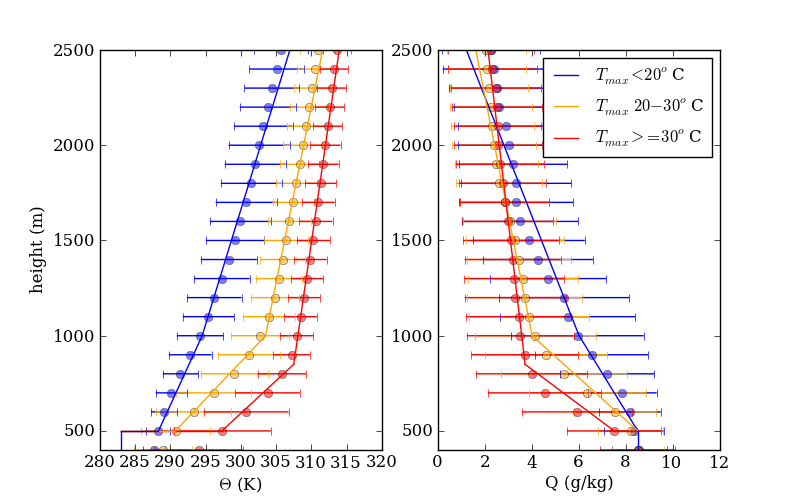
\includegraphics[width=1\textwidth]{ch2-BL/figures/fitted_lapserates_theta_Q_onefig.png}
\caption{}
\label{fig:BL_LapseRates}
\end{figure}

The range of soil moisture, free troposphere, and tree species conditions tested are listed in Table \ref{table:BL_1Druns}.  

\begin{table}
\begin{tabular}{ l c }
\hline
 & Range of values tested \\ \hline
Jarvis $VPD$ and $\theta_{rel}$ parameters & Douglas fir, Pacific madrone (Table XXX)\\
Lapse rates $\Gamma_{\Theta}$ and $\Gamma_Q$ & 1 (blue in Figure \ref{fig:BL_LapseRates}), 2 (yellow), 3 (red)\\
Relative soil moisture $\theta_{rel}$ & 0.15, 0.2, 0.25, 0.3, 0.35, 0.4, 0.45, 0.5\\
\hline
\end{tabular}
\caption{Range of values tested using the one-dimensional boundary layer model.}
\label{table:BL_1Druns}
\end{table}

\subsection{Regional climate model}
In order to further test the impact of these two tree species on the atmospheric boundary layer, we use WRF-Noah [Skamarock \textit{et al.}, 2008], a three-dimensional, non-hydrostatic regional climate model (Weather Research and Forecasting, or WRF) with terrain-following vertical coordinates and a coupled land surface model (Noah).  In WRF, the conservation equations for momentum, mass, and energy are solved numerically to calculate the temporal evolution of atmospheric state variables, including air temperature, pressure, humidity, and wind velocity.  

\begin{table}
\begin{tabular}{l l}
\hline
Scheme & Setting \\ \hline
WRF version & 3.6 \\
Grid nesting & two-way \\
Lateral boundary conditions & NCEP Eta analysis \\
Soil levels & 4 \\
Land use and soil categories & USGS \\
Land surface model & Noah \\
Surface layer & MM5 Monin-Obukhov \\
Planetary Boundary Layer (PBL) & ACM2 \\
Microphysics & WSM 3-class simple ice \\
Longwave radiation & RRTM \\
Shortwave radiation & Dudhia \\
Cumulus & Kain-Fritsch (new Eta) \\
Turbulence closure & Horizontal Smagorinzky first order \\
Momentum advection & 5th order horizontal, 3rd order vertical \\
Scalar advection & Positive definite \\
Lateral boundary & 5 grid points \\
\hline
\end{tabular}
\caption{WRF parameterization options.  See Skamarock \textit{et al.} [2008] for description of schemes.}
\label{table:BL_paramschemes}
\end{table}

Subgrid processes, including radiation, planetary boundary layer (PBL) turbulence, cloud microphysics, and convection, are parametrized in WRF, and the parametrization schemes used here are listed in Table \ref{table:BL_paramschemes}.  The ACM2 PBL scheme was used because of its ability to represent both convective regimes (non-local transport) and shear-dominated regimes (local transport) [Pleim, 2007], and because of its good performance in other WRF studies [CITATIONS including Marjanovic].

\begin{table}
\begin{tabular}{ l c c c c c c c }
\hline
Domain & $\Delta x$ (km) & $\Delta y$ (km) & $nx$ & $ny$ & $nz$ & $\Delta t$ (s) & USGS data res \\ \hline
d01 & 8.1 & 8.1 & 96 & 99 & 45 & 45 & 2 min\\
d02 & 2.7 & 2.7 & 175 & 175 & 45 & 15 & 2 min\\
\hline
\end{tabular}
\caption{Model domains. d01 refers to the outer domain, and d02 refers to the inner domain.}
\label{table:BL_domains}
\end{table}

The tests are run with two nested domains centered on the northern Coast Range (Figure XX).  The domains are two-way nested, meaning that the outer domain (d01) provides the lateral boundary conditions for the inner domain (d02), and the inner domain states are fed back to the outer domain throughout the region coincident with the inner domain.  Two-way nesting improves model accuracy, particularly in regions of complex terrain [CITATIONS].  The domain resolutions and dimensions are listed in Table \ref{table:BL_domains}.  The lateral boundaries of the outer domain are forced with NCEP Eta 212 grid (40 km) operational analysis [NCEP, 1998] for the period of 2009-08-16 00:00 to 2009-08-30 00:00, with the first 32 hours discarded as model spin-up.  This time period is rain-free and sunny at the Angelo Reserve and represents the mid- to late-summer season when soil moisture is highly limited and incoming radiation is still strong (cf. Chapter XX Figure XX - rivendell met time series).

Observed topography and USGS vegetation and soil types are used, with the exception of the northern Coast Range region highlighted in Figure XX, where the vegetation and soil types are assigned to dummy types.  The VPD and soil moisture stomatal response parameters of this dummy type are modified according to the test case as described below.  Radiative properties, leaf area, and rooting depth of the dummy type are held constant among the test cases, using the ``Evergreen Needleleaf Forest'' values.

\begin{table}
\begin{tabular}{ l p{3cm} p{3cm} p{2cm} p{3cm} }
\hline
Vegetation type & $\theta_{ref}$ (m$^3$/m$^3$) & $\theta_{wilt}$ (m$^3$/m$^3$) & RS (s/m) & HS (kg/kg)\\ \hline
ENF & 0.329 (loam) & 0.066 (loam) & 125 & 47.35\\
Douglas fir & 0.156 & 0.075 & 125 & 47.35\\
EBF & 0.329 (loam) & 0.066 (loam) & 150 & 41.69\\
Pacific madrone 1 & 0.105 & 0.047 & 550 & 10.\\
Pacific madrone 2 & 0.105 & 0.047 & 300 & 20.\\
\hline
\end{tabular}
\caption{Parameters for Noah's Jarvis formulation of stomatal conductance, by vegetation type.  RS is the Noah minimum stomatal resistance parameter in the Jarvis formulation. HS is the Noah scaling factor for the specific humidity deficit in the Jarvis humidity stress function (Equation XX). ENF is the USGS Evergreen Needleleaf Forest land use type; EBF is the USGS Evergreen Broadleaf Forest land use type.}
\label{table:BL_NoahJarvisparams}
\end{table}

\begin{table}
\begin{tabular}{ l p{6cm} p{7cm} }
\hline
Run ID & VPD parameters (RS, HS) & Soil moisture parameters ($\theta_{ref}$, $\theta_{wilt}$)\\ \hline
vDF-sDF & Douglas fir (ENF) & Douglas fir\\
vEBF-sMD & EBF & Pacific madrone\\
vMD1-sMD & Pacific madrone 1 & Pacific madrone\\
vMD2-sMD & Pacific madrone 2 & Pacific madrone\\
\hline
\end{tabular}
\caption{Combinations of stomatal conductance Jarvis parameters used in the WRF tests.  Each pair of parameters is tested for a range of volumetric soil moisture values in the northern Coast Range test region: 0.08, 0.1, 0.12, and 0.14 m$^3$/m$^3$.}
\label{table:BL_WRFruns}
\end{table}

The Noah model uses a Jarvis formulation of stomatal conductance similar to that used in Chapter XX (Equation XX).  The XX parameter is the minimum stomatal resistance (equivalent to $1/g_s$), and XX is divided by empirical functions of environmental variables.  The soil moisture stress function is the piecewise-linear, threshold Feddes model [\textit{Feddes et al.}, 1978; \textit{Chen et al.}, 2008].  The parameters for the sigmoid model from Chapter XX (Equation XX, Table XX) thus must be translated to the Feddes parameters (reference or stress point, $\theta_{ref}$, and wilting point, $\theta_{wilt}$).  For each species, we fit a line to $f_{\theta}$ between $f_{\theta}=0.05$ and $f_{\theta}=0.95$ and extrapolate the line to 0 to estimate $\theta_{wilt}$ and to 1 to estimate $\theta_{ref}$ (Figure \ref{fig:BL_FeddesParams}, Table \ref{table:BL_NoahJarvisparams}).


Soil moisture in the Coast Range test region is reset each day at midnight local time, so that the soil moisture deviates only minimally from its stated value (e.g. Figure XX shows one of the wettest cases, XXXX, with a daily decline of XX m$^3$/m$^3$ or less).

The empirical function representing humidity stress is similar to the \textbf{Lohammar} function used in Chapter XX (Equation XX):

\textbf{WRF Q EQUATION}

The $1/rsmin * f(VPD)$ using USGS parameters for Evergreen Needleleaf Forest (ENF, COLOR) and Evergreen Broadleaf Forest (EBF, COLOR) are shown in Figure XX (top panel).  For comparison, the $g_{s, max}/\alpha * f(VPD)$ calculated using sap-flow-derived species averaged parameters for Douglas fir and Pacific madrone (Chapter XX, Table XX) are also shown in Figure XX (bottom panel).  The ENF and Douglas fir $g_s$ respond very similarly to humidity stress, so the existing ENF parameters are used to represent the Douglas fir.  The model EBF $g_s$ is much higher than is the Pacific madrone $g_s$ at low $VPD$ (relative to ENF or Douglas fir, respectively).  As such, we run tests with the EBF VPD parameters representing Pacific madrone (parameters listed in Table \ref{table:BL_NoahJarvisparams}; runs TEST NAMES, Table XX), but we also test two additional rsmin-hs parameter pairs that more closely approximate the shape of the sap-flow-derived curve for Pacific madrone (COLORS lines in Figure XX; parameters listed in Table \ref{table:BL_NoahJarvisparams}; runs TEST NAMES, Table XX).

\begin{figure}[here]
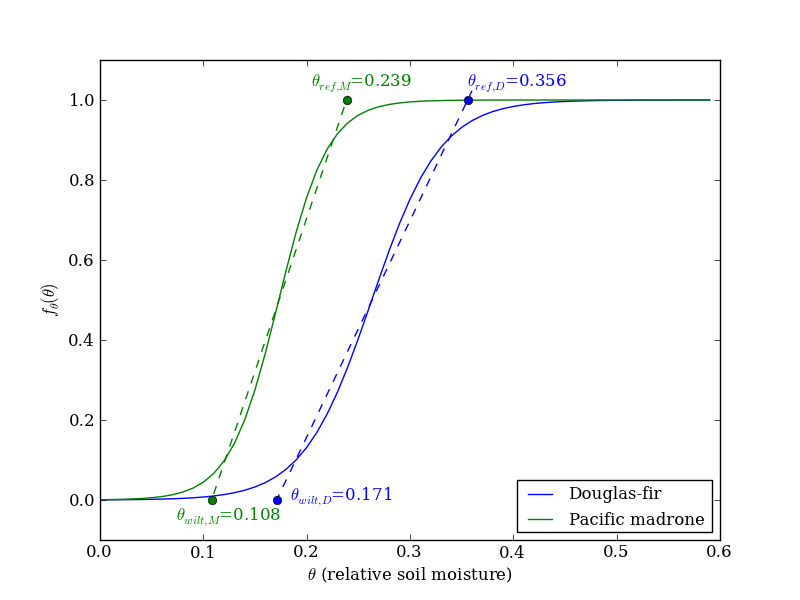
\includegraphics[width=1\textwidth]{ch2-BL/figures/theta_params.png}
\caption{}
\label{fig:BL_FeddesParams}
\end{figure}


WRF-Noah is run using the permutations of stomatal response parameters listed in Table \ref{table:BL_NoahJarvisparams}, with a range of soil moisture values (0.08, 0.1, 0.12, 0.14).  These values are equivalent to relative soil moistures of XXXX, given that the saturation moisture content of the loam soil type used in the model is 0.439 m$^3$/m$^3$.  These relative soil moisture values span the range of values observed in August at the Angelo Coast Range Reserve (Chapter XX, Figure XX).

\section{Results}

\subsection{1-D model}

\begin{figure}[here]
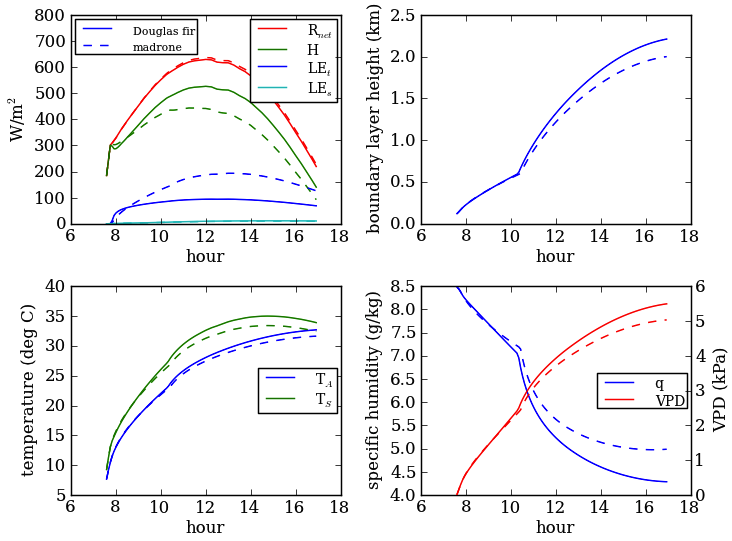
\includegraphics[width=0.9\textwidth]{ch2-BL/figures/testall_Aug15_soilm0pt25_ra10_lapseT2_cropped.png}
\caption{Diurnal cycle simulated by 1-D model for $\theta_{rel}=0.25$ and lapse rate \#2.  Solid lines: Douglas fir case; dashed lines: Pacific madrone case.  Top left: surface energy flux terms ($R_{net}$ is net radiation, $H$ is sensible heat, $LE_t$ is latent heat due to transpiration, and $LE_s$ is latent heat due to soil evaporation.)  Top right: boundary layer height.  Bottom left: surface temperature ($T_S$) and mixed layer air temperature ($T_A$) adjusted to 400 m ASL (ground level in ACRR).  Bottom right: mixed layer specific humidity ($q$) and $VPD$.}
\label{fig:BL_1Ddiurnal}
\end{figure}

The 1-D model simulates a reasonable diurnal cycle for mid-August, but with temperatures several degrees higher than observations at the ACRR, which may result from using tropospheric soundings from Oakland.  Figure \ref{fig:BL_1Ddiurnal} shows a typical diurnal cycle for a moderate lapse rate (\#2) and relative soil moisture $\theta_{rel} = 0.25$.  The Pacific madrone forest has higher transpiration than the Douglas fir forest, because Pacific madrone stomatal conductance is higher at this value of $\theta_{rel}$ (c.f. Figure \ref{fig:BL_FeddesParams}); both cases have very little soil evaporation at this value of $\theta_{rel}$.  As a result, the Pacific madrone case has lower sensible heat ($H$) than the Douglas fir case, leading to a shallower, cooler, and moister boundary layer over the Pacific madrone forest.

\begin{figure}[here]
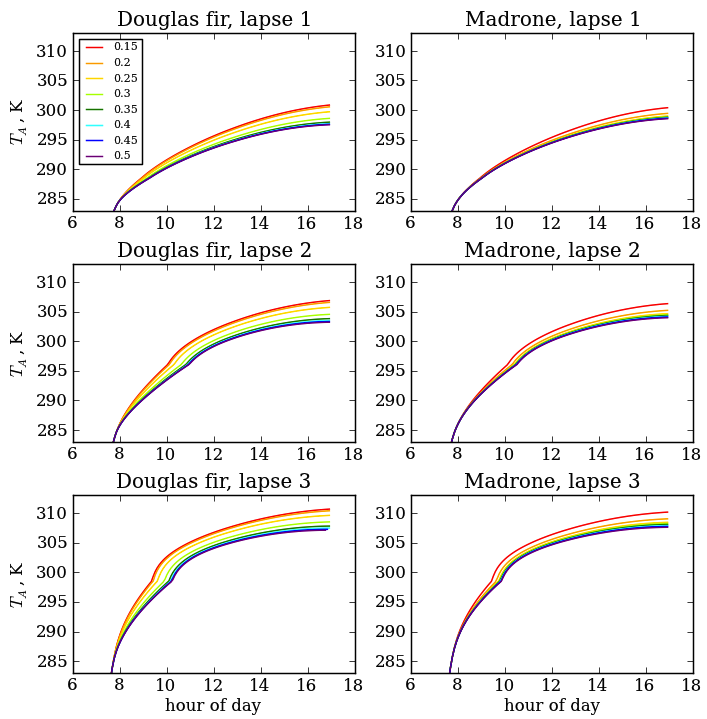
\includegraphics[width=0.9\textwidth]{ch2-BL/figures/testall_compare_sm_lapse_Ta_cropped.png}
\caption{Diurnal cycle of air temperature at 400 m ASL (ground level in ACRR), simulated by the 1-D model, for a range of $\theta_{rel}$ (colors) and free troposphere conditions.  Left column: Douglas fir case; right column: Pacific madrone case.  Top row: lapse rate 1 (coolest free troposphere conditions); middle row: lapse rate 2 (moderate free troposphere conditions); bottom row: lapse rate 3 (warmest free troposphere conditions).}
\label{fig:BL_1DdiurnalTa}
\end{figure}

\begin{figure}[here]
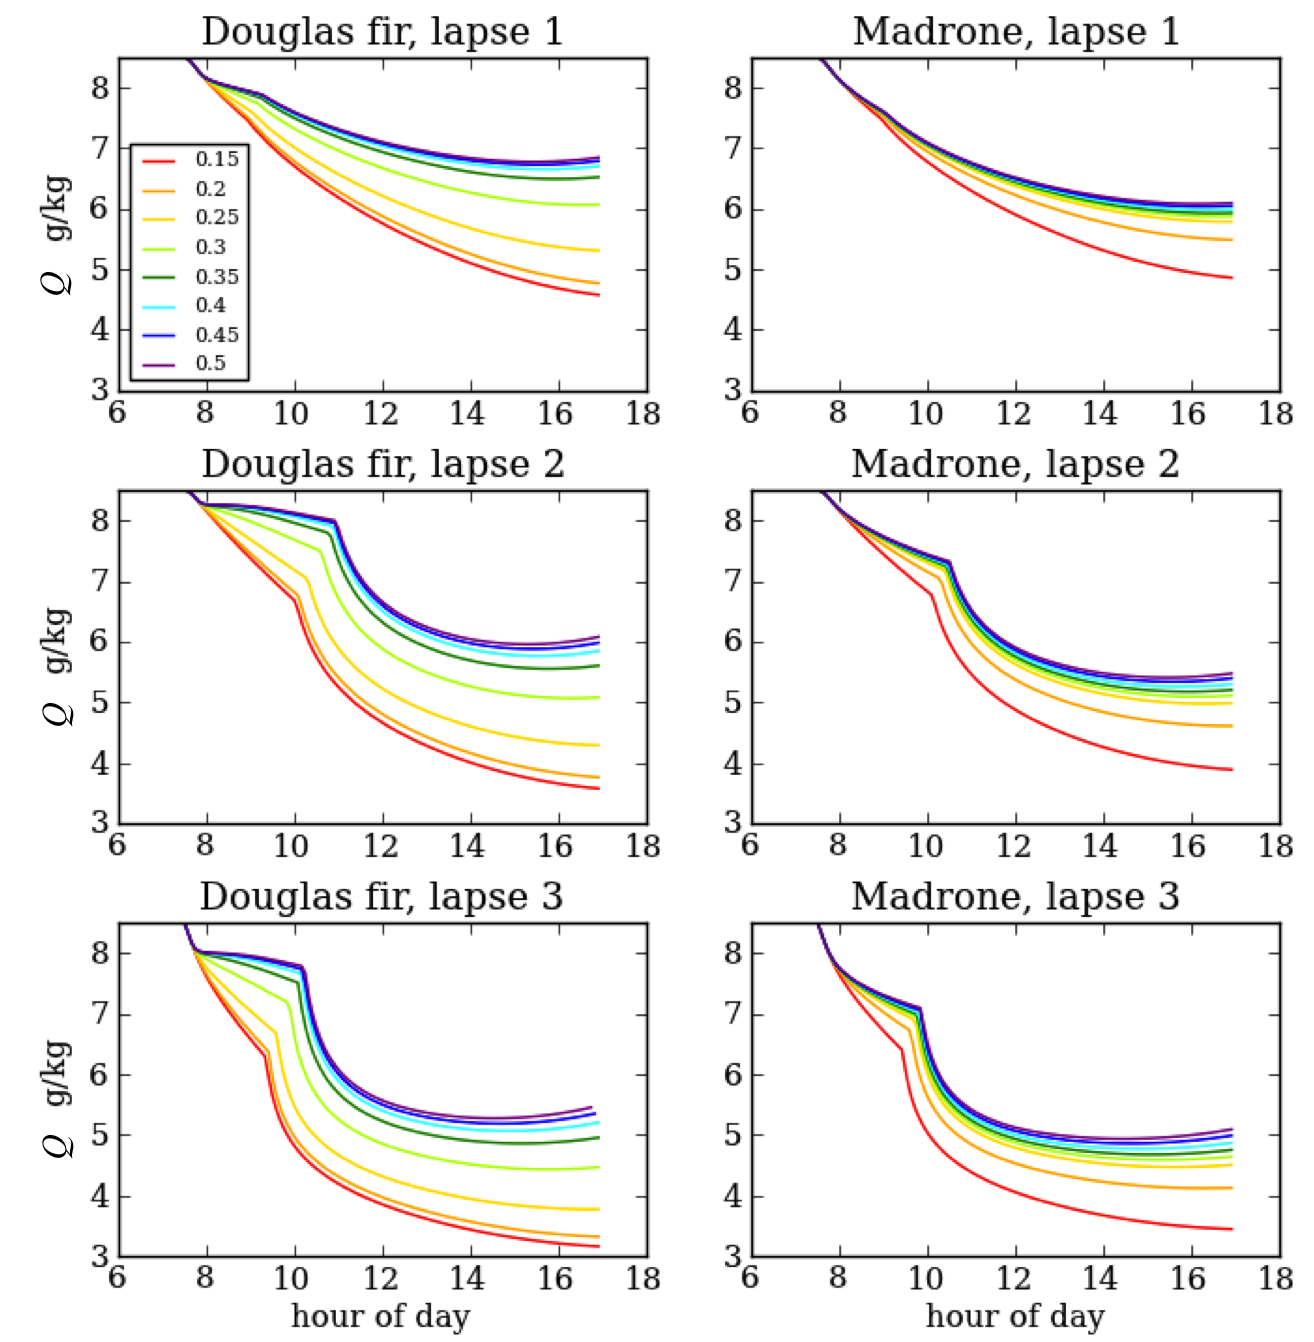
\includegraphics[width=0.9\textwidth]{ch2-BL/figures/testall_compare_sm_lapse_Q_cropped2.png}
\caption{Diurnal cycle of boundary layer specific humidity, simulated by the 1-D model, for a range of $\theta_{rel}$ (colors) and free troposphere conditions.  Left column: Douglas fir case; right column: Pacific madrone case.  Top row: lapse rate 1 (most moist free troposphere conditions); middle row: lapse rate 2 (moderate free troposphere conditions); bottom row: lapse rate 3 (driest free troposphere conditions).}
\label{fig:BL_1DdiurnalQ}
\end{figure}

%\clearpage

The boundary layer is warmer and drier when the free troposphere is warmer and drier (Figures \ref{fig:BL_1DdiurnalTa} and \ref{fig:BL_1DdiurnalQ}; increasing $T_a$ and decreasing $Q$ from lapse rate 1 to 2 to 3).  Additionally, the shape of the diurnal cycle differs among the free troposphere cases, with most rapid morning increase in $T_a$ in the hottest case (lapse rate 3), due to entrainment of high-$\Theta$ air in the steep low-level inversion.  The drier free troposphere conditions in lapse rate 3 also lead to lower $Q$, but with a slower morning decline of $Q$ because of relatively slow boundary layer growth through the steep inversion.

\begin{figure}[here]
\begin{subfigure}{0.5\textwidth}
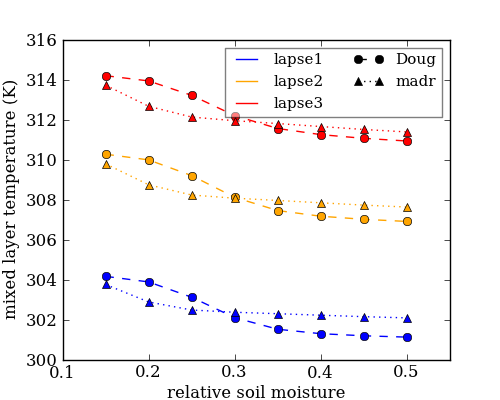
\includegraphics[width=\textwidth]{ch2-BL/figures/all_afternoon_T.png}
\caption{}
\end{subfigure}
\begin{subfigure}{0.5\textwidth}
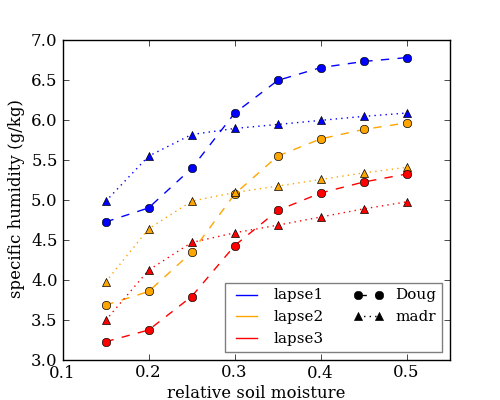
\includegraphics[width=\textwidth]{ch2-BL/figures/all_afternoon_Q.png}
\caption{}
\end{subfigure}
\caption{Conditions at 3:45 pm in the 1-D model, as a function of soil moisture, for the three free troposphere lapse rates (colors).  (a) Air temperature at 400 m ASL (ground level in ACRR), and (b) specific humidity.  Dashed lines with circles: Douglas fir case.  Dotted lines with triangles: Pacific madrone case.}
\label{fig:BL_345changes}
\end{figure}

%\clearpage

For both the Pacific madrone forest and the Douglas fir forest, drier soil (decreasing $\theta_{rel}$) leads to a warmer and drier boundary layer (increasing $T_a$ and decreasing $Q$).  However, in the Douglas fir case, the increase in $T_a$ and decrease in $Q$ begin when the soil is wetter ($\theta_{rel} \le 0.3$; Figures \ref{fig:BL_1DdiurnalTa} and \ref{fig:BL_1DdiurnalQ}, left columns), while in the Pacific madrone case, the increase in $T_a$ and decrease in $Q$ begin only when soil is drier ($\theta_{rel} \le 0.2$; Figures \ref{fig:BL_1DdiurnalTa} and \ref{fig:BL_1DdiurnalQ}, right columns).  

The differences between the species cases are largest in the afternoon; Figure \ref{fig:BL_345changes} shows $T_a$ and $Q$ at 3:45 pm for the Douglas fir and Pacific madrone cases, as a function of $\theta_{rel}$ and free troposphere conditions.  The differences between the Douglas fir and Pacific madrone cases for both $T_a$ and $Q$ are largest at $\theta_{rel}$ values around 0.2, with the Douglas fir case hotter by 1-1.5 $^\circ$C and drier by $\sim$0.7 g/kg.  A $\theta_{rel}$ value of 0.2-0.25 is typical for the mid- to late-dry-season at the ACRR (Figure \ref{fig:sapflow_met}). Interestingly, at $\theta_{rel}$ values higher than about 0.35, the Douglas fir case is actually cooler and moister; such $\theta_{rel}$ values are typical for the late spring and early summer at the ACRR (Figure \ref{fig:sapflow_met}).

\begin{figure}[here]
\begin{subfigure}{0.5\textwidth}
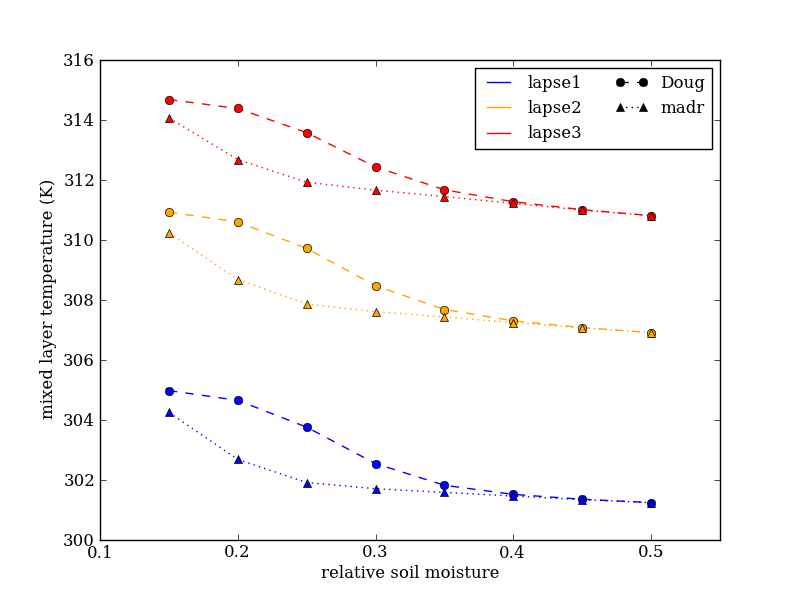
\includegraphics[width=\textwidth]{ch2-BL/figures/theta_afternoon_T.png}
\caption{}
\end{subfigure}
\begin{subfigure}{0.5\textwidth}
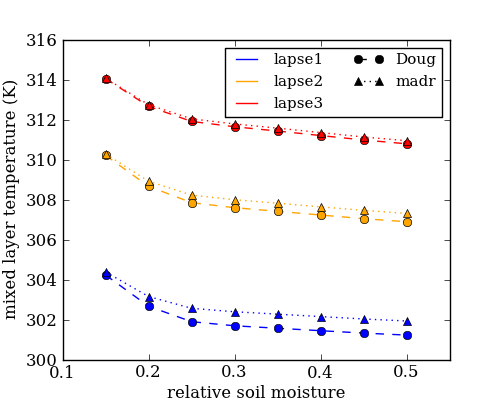
\includegraphics[width=\textwidth]{ch2-BL/figures/VPD_afternoon_T.png}
\caption{}
\end{subfigure}
\caption{Air temperature at 400 m ASL (ground level in ACRR) at 3:45 pm in the 1-D model, as a function of soil moisture, for the three free troposphere lapse rates (colors).  (a) holding $VPD$ parameters constant at Douglas fir values and varying $\theta$ parameters by species, and (b) holding $\theta$ parameters constant at Pacific madrone values and varying $VPD$ parameters by species.}
\label{fig:BL_testVPDtheta}
\end{figure}

The temperature and humidity differences at $\theta_{rel} \le 0.3$ are due largely to Douglas firs' greater stomatal closure with dry soil.  Model tests setting the $VPD$ parameters ($D_o$ and $g_{c,max}$) to the Douglas fir values (Table \ref{tbl:sapflow_mcmc}) and varying the $\theta$ parameters ($\theta_0$ and $\beta$) by species give a Douglas fir - Pacific madrone temperature difference of 1.5-2$^\circ$C at $\theta_{rel} = 0.2$ (Figure \ref{fig:BL_testVPDtheta}(a)), while tests setting the $\theta$ parameters to the Pacific madrone values and varying the $VPD$ parameters by species give a temperature difference of \textless 0.5$^\circ$C at $\theta_{rel} = 0.2$ (Figure \ref{fig:BL_testVPDtheta}(b)).  Thus, in dry soil, the Douglas fir $VPD$ response does little to moderate the temperature differences caused by Douglas fir stomatal closure at low $\theta_{rel}$.  However, in wet soils ($\theta_{rel}$ \textless $0.3$), and particularly in cool free troposphere conditions, the greater Douglas fir stomatal conductance at low $VPD$ cools the boundary layer (Figure \ref{fig:BL_testVPDtheta}(b)), while soil moisture plays little role (Figure \ref{fig:BL_testVPDtheta}(a)).

%- fraction of moisture from land surface vs. from free troposphere, for different soil moisture / lapse rate / species conditions

\subsection{Regional climate model}

\begin{figure}[here]
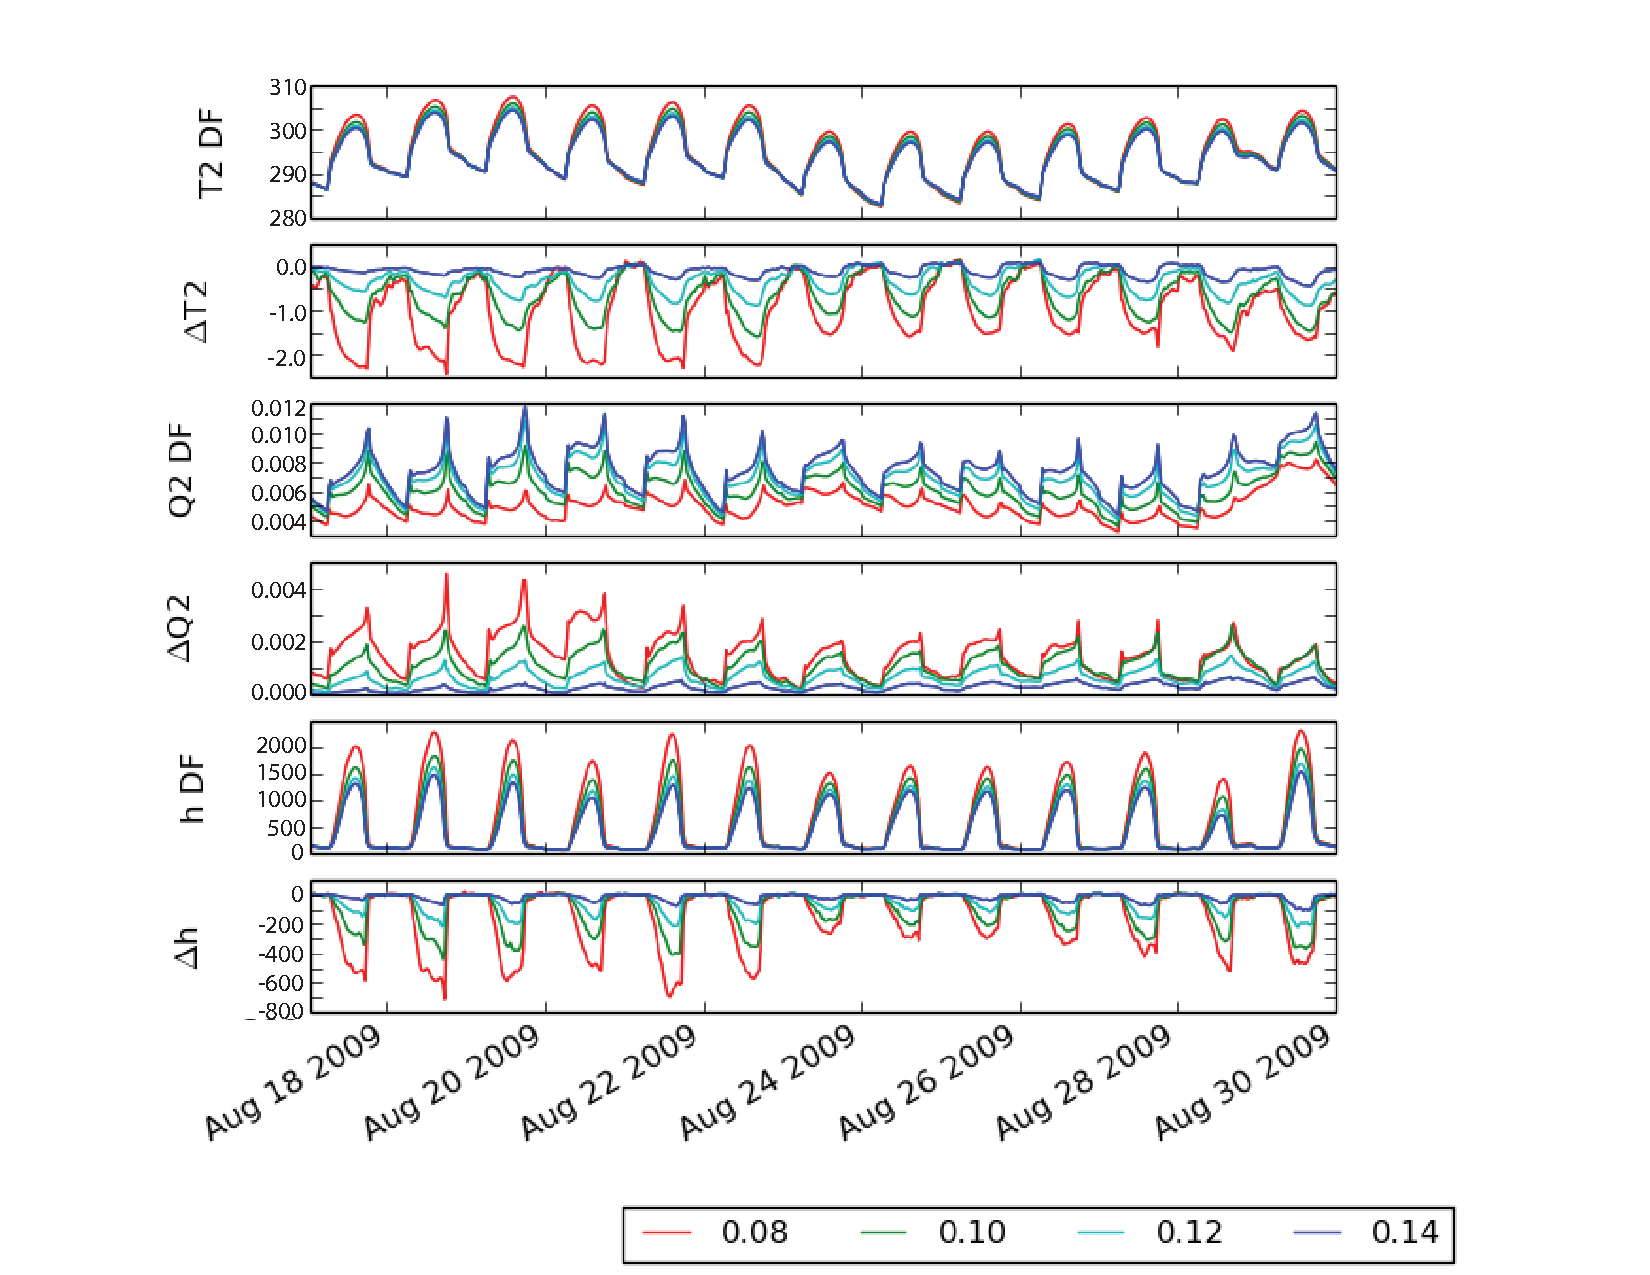
\includegraphics[width=\textwidth]{ch2-BL/figures/T_Q_h_d02.pdf}
\caption{Time series of near-surface conditions in the WRF tests, averaged over the test region, for a range of $\theta_{vol}$ values (colors).  Top panel: air temperature (K) at 2 m above ground level for the all-Douglas-fir case.  Second panel: difference in 2 m air temperature between the all-Pacific-madrone case and the all-Douglas-fir case.  Third panel: specific humidity ($q$, kg/kg) at 2 m above ground, for the all-Douglas-fir case.  Fourth panel: difference in 2 m $q$ between the all-Pacific-madrone case and the all-Douglas-fir case.  Fifth panel: boundary layer height in the all-Douglas-fir case.  Sixth panel: difference in boundary layer height between the all-Pacific-madrone case and the all-Douglas-fir case.}
\label{fig:BL_WRFtseries}
\end{figure}

Figure \ref{fig:BL_WRFtseries} shows the time series of atmospheric conditions averaged over the test region in the Douglas fir case (panels 1, 3, and 5) and the difference between the Pacific madrone and Douglas fir case (panels 2, 4, and 6).  In the Douglas fir case, drier soils lead to a hotter (panel 1 of Figure \ref{fig:BL_WRFtseries}), drier (panel 3), and deeper (panel 5) boundary layer than do wet soils.  For soil moisture $\le$ 0.12 m$^3$/m$^3$ ($\theta_{rel} \le 0.27$), the boundary layer over the madrone forest is cooler (panel 2), moister (panel 4), and shallower (panel 6) than that over the Douglas fir forest; the differences are negligible for soil moisture of 0.14 m$^3$/m$^3$ ($\theta_{rel} = 0.32$).  The differences between the species cases increase with drier soil: the greatest differences occur when soil moisture is 0.08 m$^3$/m$^3$, with 2 m air temperature in the madrone case cooler by 1.5-2.5$^\circ$C, 2 m humidity greater by 1-3 g/kg, and boundary layer depth shallower by 200-500 m, averaged over the test region.

\begin{figure}[here]
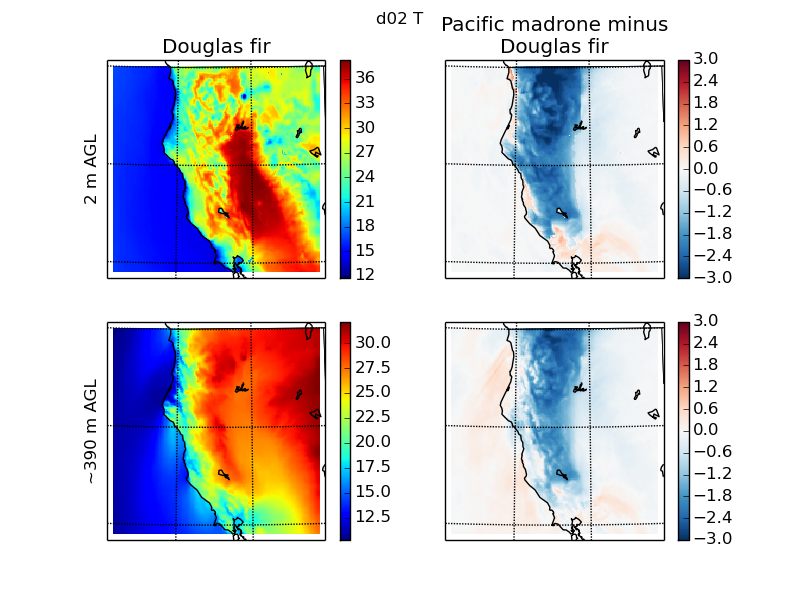
\includegraphics[width=1\textwidth]{ch2-BL/figures/T_d02_s0pt08.png}
\caption{Left column: temperature ($^\circ$C) in domain d02 for the Douglas fir case.  Right column: temperature difference between the Pacific madrone case and the Douglas fir case.  Top row: 2 m above ground level (AGL).  Bottom row: model level at $\sim$390 m AGL (380-395 m for the test region).}
\label{fig:BL_WRFmapT}
\end{figure}

\begin{figure}[here]
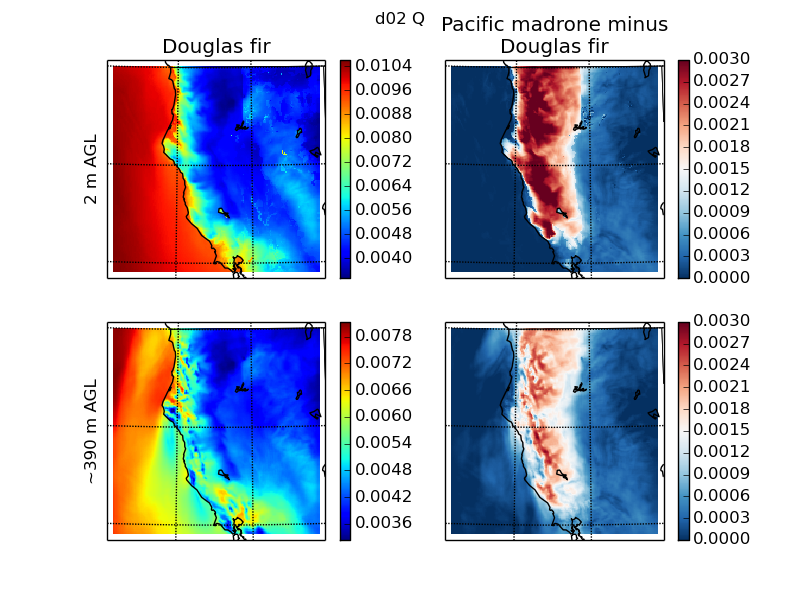
\includegraphics[width=1\textwidth]{ch2-BL/figures/Q_d02_s0pt08.png}
\caption{Left column: specific humidity (kg/kg) in domain d02 for the Douglas fir case.  Right column: specific humidity difference between the Pacific madrone case and the Douglas fir case.  Top row: 2 m AGL.  Bottom row: model level at $\sim$390 m AGL (380-395 m for the test region).}
\label{fig:BL_WRFmapQ}
\end{figure}

\begin{figure}[here]
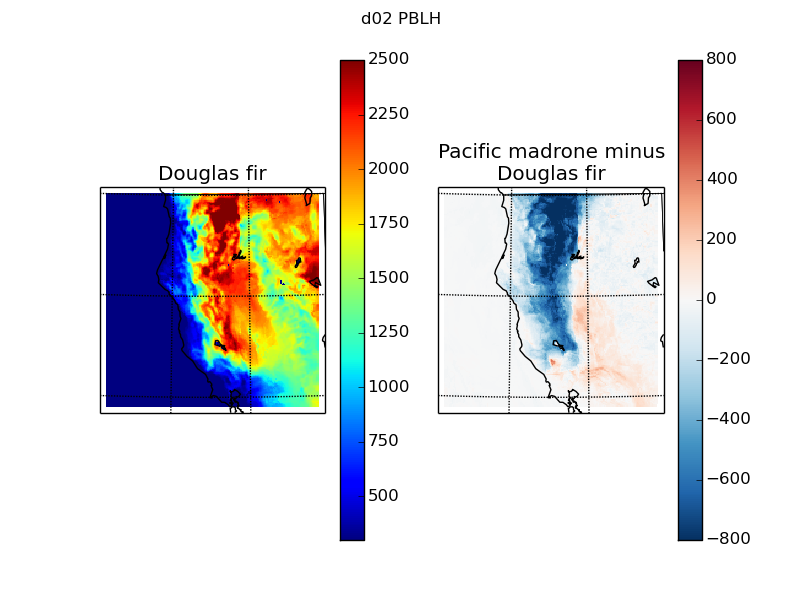
\includegraphics[width=1\textwidth]{ch2-BL/figures/PBLH_d02_s0pt08.png}
\caption{Left column: boundary layer height (m) in domain d02 for the Douglas fir case.  Right column: boundary layer height difference (m) between the Pacific madrone case and the Douglas fir case.}
\label{fig:BL_WRFmapPBLH}
\end{figure}

The differences in temperature and humidity persist from 2 m AGL (Figures \ref{fig:BL_WRFmapT} and \ref{fig:BL_WRFmapQ}, top rows) through to the mixed layer at $\sim$390 m AGL (Figures \ref{fig:BL_WRFmapT} and \ref{fig:BL_WRFmapQ}, bottom rows). The species differences are smaller at 390 m AGL than at 2 m AGL: the madrone case is cooler than the Douglas fir case by up to $\sim$2.5$^\circ$C at 2 m AGL and by up to $\sim$1.5$^\circ$C at 390 m AGL; humidity in the madrone case is greater than in the Douglas fir case by 2-3 g/kg at 2 m AGL and by 1.5-2.5 g/kg at 390 m AGL.

The changes in 390 m AGL temperature and humidity and in boundary layer depth are greatest inland, where the convective boundary layer is fully developed.  The boundary layer in the control Douglas fir case is shallow near the coast but deepens inland (Figure \ref{fig:BL_WRFmapPBLH}, left panel), as expected from previous analytical and numerical studies [\cite{garratt1990internal}].  Because the boundary layer is shallow in this zone, the differences in surface energy balance between the species cases may not be fully communicated to an altitude of 390 m AGL.  The deeper boundary layer inland means that the air at 390 m AGL is part of the mixed layer that communicates rapidly with the surface; thus, the changes in temperature and humidity in the madrone case affect the air at 390 m AGL over inland but not coastal regions.




\section{Discussion and Conclusions}

Large-scale conversion of the northern California Coast Range forest from all-Douglas-fir to all-Pacific-madrone cools and moistens the summertime boundary layer when relative soil moisture is less than 0.3, conditions typical of late summer at the ACRR (Figure \ref{fig:sapflow_met}).   Two atmospheric models, one simple and one complex, simulate a cooling of $\sim$1.5$^\circ$C in the mixed layer ($\sim$2.5$^\circ$C near the surface) and a moistening of 1 g/kg in the mixed layer (2-3 g/kg near the surface).  With 100\% Pacific madrone coverage compared with 100\% Douglas fir coverage, Pacific madrone cools and moistens the boundary layer when soils are dry because madrone stomatal conductance and thus transpiration remains higher at low soil moisture.  The greater transpiration consumes a larger fraction of net radiation in latent heat and reduces the sensible heat flux; because sensible heat is reduced, there is less direct heating of the boundary layer from the surface, and there is less entrainment of the hotter, drier free tropospheric air above the boundary layer.

The simple model and the complex model estimate similar magnitudes of temperature and humidity differences between the Douglas fir and Pacific madrone cases; the similarity of the results confirms the role of evapotranspiration in the near-surface atmosphere in the northern California Coast Range, especially in the dry season.  The 1-D boundary layer model does not include the effects of advection or subsidence and thus overestimates boundary layer height and temperature at the ACRR field site; however, the differences in temperature and humidity between the Douglas fir and Pacific madrone cases simulated by the simple model agree with the differences simulated by the complex model.  Even accounting for the effects of advection, complex topography, and subsidence in WRF, the hotter and drier conditions of the Douglas fir case relative to the Pacific madrone case are a robust result.

The differences in late summer temperature and humidity are due largely to the differences in stomatal response to soil water deficit (Figure \ref{fig:BL_testVPDtheta}).  Importantly, WRF does not represent vegetation-type differences in stomatal response to soil moisture; rather, the $\theta_{ref}$ and $\theta_{wilt}$ parameters depend only on soil type in WRF.  This inability to represent vegetation differences in water stress points prevents WRF from accurately representing the variation in land surface response to drought.  Adding vegetation-type-specific $\theta_{ref}$ and $\theta_{wilt}$ parameters to the WRF Noah land surface model would improve WRF's ability to simulate ecosystem-atmosphere interactions.

While we incorporate sap-flow-derived parameters for stomatal response to soil moisture in both models, in the WRF tests we do not use sap-flow-derived parameters for the $VPD$ response.  In order to incorporate sap-flow-derived $VPD$ parameters into WRF in future work, measurements of the sapwood area to leaf area ratio are necessary (for converting $g_{s,max}$, representing conductance on a per-sapwood-area basis, to $1/RS$, representing stomatal conductance on a per-leaf-area basis).  The sap-flow-based $VPD$ parameters should also be re-estimated using $\Delta q$ instead of $VPD$, in accord with the WRF humidity stress function (Equation \ref{eqn:BL_WRFq}).  Nevertheless, the effect of differences in $VPD$ parameters is small when $VPD$ is high and soil is dry, as is the case in mid- to late-summer (Figure \ref{fig:BL_testVPDtheta}).  The effect of differences in $VPD$ parameters may be larger when soil is wet and $VPD$ is low to moderate, as in winter and spring; simulations of those conditions would require more accurate estimation of species-specific $VPD$ parameters.

Using sap flow measurements to parameterize a regional climate model requires a significant scale jump, from the scale of whole trees and a single hillslope, to the scale of 2.7 km grid boxes and a 500 km x 500 km domain.  Such scale jumps are inherent in the measurement of evapotranspiration; however, further sap flow measurements of these species on slopes with different aspects, elevations, and species mixes are needed in order better to quantify the variability in stomatal response parameters and covariation with other environmental conditions.

The regional cases tested here are extreme scenarios involving the total conversion of the forest from one species (Douglas fir) to the other (Pacific madrone).  However, this may not be wholly unrealistic: Pacific madrones were likely more abundant in the past, due to regular controlled burning by indigenous people [\cite{johnsonACRR}].  It is possible that longer and more severe droughts in a warmer future climate could cause a shift from Douglas fir to Pacific madrone, if fires become more frequent and if Douglas firs are less tolerant of drought.  Moreover, forest management stakeholders are actively discussing controlling the encroachment of Douglas fir in this region [William Dietrich, personal communication]. This study demonstrates that such regional-scale species shifts could have regional-scale impacts on air temperature and humidity in the dry season.

In this study, we integrate tree-scale field observations with physical atmospheric models to test regional atmospheric feedbacks of species-specific stomatal behavior.  We demonstrate the sensitivity of the boundary layer to stomatal dynamics and show that a regional-scale change in dominant evergreen tree species can change summertime afternoon near-surface temperatures by $\sim$2$^\circ$C.  This result underscores the importance of understanding species- and vegetation-type-differences in stomatal response to soil moisture and $VPD$.
